\clearpage

\chapter{Title of Third Manuscript}
\label{chapter:05_manuscript_III}

\section{Chapter Overview}
This chapter presents a synthesis of research experiments reported in a manuscript... 
\Blindtext[1]

The manuscript reference is provided below:

\vspace{1em}

\noindent Smith J. Robust calibration for noisy sensor networks. \textit{International Journal of Applied Signal Processing.} 2024;19(3):201-214.

\section{Abstract}

\noindent \Blindtext[1][2]
\clearpage

\section{Introduction}

\Blindtext[1]

\subsection{Background and Rationale}

\Blindtext[1]

\subsection{Related Work}

\Blindtext[1]

\subsection{Research Objectives}

The goal of this chapter is... :

\begin{enumerate}
    \item First objective
    \item Second objective 
    \item Third objective
\end{enumerate}

\Blindtext[1]

\subsection{Research Questions}

This chapter addresses the following research questions...:

\begin{enumerate}
    \item First research question
    \item Second research question
    \item Third research question
\end{enumerate}

The findings of this work aim to...
\Blindtext[1]

\section{Methods}
Detail datasets, selection rules, and analysis steps. Provide enough information for replication \cite{smith2021method}. Reference algorithms as Algorithm~\ref{alg:ms3_algorithm}.

\begin{algorithm}[htbp]
\caption{Creating rolling-window features from time-series sensor data for a regression model.}
\label{alg:ms3_algorithm}
    \begin{algorithmic}[1]
    \Require DataFrame \texttt{df}, time column \texttt{tcol}, value column \texttt{vcol}, window size \texttt{w}, step size \texttt{s}
    \State sort \texttt{df} by \texttt{tcol} in ascending order
    \State \textbf{Procedure} make\_window\_features(window values)
        \Indent
            \If{any missing values in \texttt{window}}
                \State fill missing values using forward fill, then backward fill
            \EndIf
            \State \texttt{mean} $\gets$ average of \texttt{window}
            \State \texttt{std} $\gets$ standard deviation of \texttt{window}
            \State \texttt{min} $\gets$ minimum of \texttt{window}
            \State \texttt{max} $\gets$ maximum of \texttt{window}
            \State \texttt{slope} $\gets$ least-squares slope of \texttt{window} vs. index
            \State \Return \{\texttt{mean}, \texttt{std}, \texttt{min}, \texttt{max}, \texttt{slope}\}
        \EndIndent
    \State \texttt{features} $\gets$ empty list
    \State \texttt{targets} $\gets$ empty list
    \For{\texttt{i} $\gets 0$ to \texttt{len(df)} $- w - 1$ step \texttt{s}}
        \State \texttt{window\_df} $\gets$ rows \texttt{i} to \texttt{i + w - 1} of \texttt{df}
        \State \texttt{window} $\gets$ values from \texttt{window\_df[vcol]}
        \State \texttt{x} $\gets$ make\_window\_features(\texttt{window})
        \State \texttt{y} $\gets$ value of \texttt{df[vcol]} at row \texttt{i + w}
        \State append \texttt{x} to \texttt{features}
        \State append \texttt{y} to \texttt{targets}
    \EndFor
    \State \texttt{X} $\gets$ DataFrame from \texttt{features} with columns \texttt{f\_mean}, \texttt{f\_std}, \texttt{f\_min}, \texttt{f\_max}, \texttt{f\_slope}
    \State \texttt{y} $\gets$ Series from \texttt{targets}, aligned with \texttt{X.index}
    \State \texttt{out\_df} $\gets$ concatenate \texttt{X} and \texttt{y} along axis 1
    \Return \texttt{out\_df}
    \end{algorithmic}
\end{algorithm}


\section{Results}

Tables can span \texttt{\textbackslash textwidth} using \texttt{tabularx} as in Table~\ref{tab:ms3_tabularx}. Figure~\ref{fig:ms3_four_panel} summarizes the four-panel comparison, with representative examples shown in each quadrant. The top-row views in Figures~\ref{fig:ms3_top_left}, ~\ref{fig:ms3_top_right} highlight the primary differences between conditions, while Figure~\ref{fig:ms3_bottom_left} provides a complementary baseline. Taken together, Figures~\ref{fig:ms3_top_left}--\ref{fig:ms3_bottom_right} show the full set of outcomes across all four panels. Figure~\ref{fig:ms3_dummy_diurnal_demand} shows an example of using the \texttt{\textbackslash begin\{axis\}} environment in TikZ/pgfplots.

\begin{figure}[H]
  \centering
  % Top row
  \begin{subfigure}[t]{0.48\textwidth}
    \includegraphics[width=\linewidth, keepaspectratio]{example-image}
    \caption{Top left}
    \label{fig:ms3_top_left}
  \end{subfigure}
  \hfill
  \begin{subfigure}[t]{0.48\textwidth}
    \includegraphics[width=\linewidth, keepaspectratio]{example-image}
    \caption{Top right}
    \label{fig:ms3_top_right}
  \end{subfigure}
  \vspace{1em}
  % Bottom row
  \begin{subfigure}[t]{0.48\textwidth}
    \includegraphics[width=\linewidth, keepaspectratio]{example-image}
    \caption{Bottom left}
    \label{fig:ms3_bottom_left}
  \end{subfigure}
  \hfill
  \begin{subfigure}[t]{0.48\textwidth}
    \includegraphics[width=\linewidth, keepaspectratio]{example-image}
    \caption{Bottom right}
    \label{fig:ms3_bottom_right}
  \end{subfigure}
  \caption{Panel of four images using the built-in `example-image` from the graphicx package}
  \label{fig:ms3_four_panel}
\end{figure}



\begin{figure}[htbp]
\centering
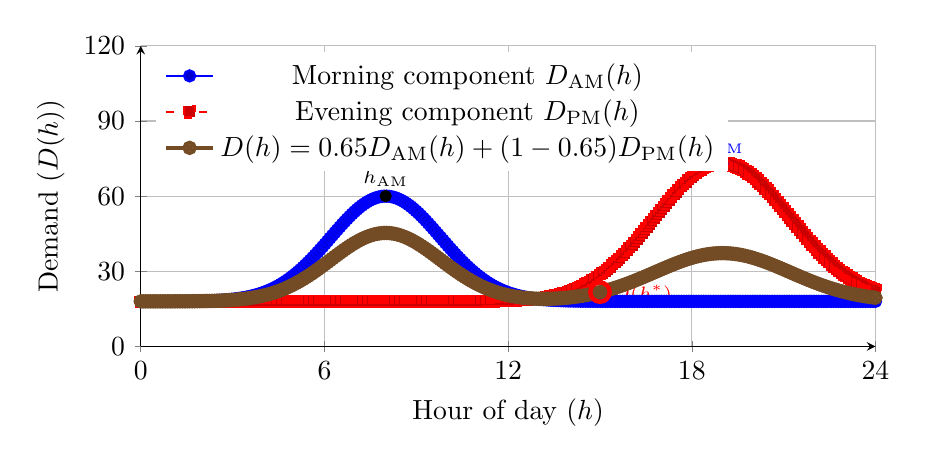
\begin{tikzpicture}
\begin{axis}[
  width=0.9\linewidth, height=5.4cm,
  xmin=0, xmax=24, ymin=0, ymax=120,
  axis lines=left,
  xlabel={Hour of day ($h$)}, ylabel={Demand ($D(h)$)},
  xtick={0,6,12,18,24},
  ytick={0,30,60,90,120},
  legend style={draw=none, at={(0.02,0.98)}, anchor=north west},
  clip=true,
  grid=both,
]

\pgfmathdeclarefunction{bump}{3}{%
  \pgfmathparse{#1*exp(-0.5*((x-#2)/#3)^2)}%
}

\def\base{18}
\def\ampM{42} \def\muM{8}  \def\sigM{1.8}
\def\ampE{55} \def\muE{19} \def\sigE{2.2}
\def\alpha{0.65}

% Precompute marker y-values (so coordinates are plain numbers)
\pgfmathsetmacro{\yM}{\base+\ampM}
\pgfmathsetmacro{\yE}{\base+\ampE}

\addplot+[domain=0:24, samples=300, thick] {\base + bump(\ampM,\muM,\sigM)};
\addlegendentry{Morning component $D_{\mathrm{AM}}(h)$}

\addplot+[domain=0:24, samples=300, thick, dashed] {\base + bump(\ampE,\muE,\sigE)};
\addlegendentry{Evening component $D_{\mathrm{PM}}(h)$}

\addplot+[domain=0:24, samples=300, very thick]
  {\alpha*(\base + bump(\ampM,\muM,\sigM)) + (1-\alpha)*(\base + bump(\ampE,\muE,\sigE))};
\addlegendentry{$D(h)=\alpha D_{\mathrm{AM}}(h)+(1-\alpha)D_{\mathrm{PM}}(h)$}

\addplot+[mark=*, only marks] coordinates {(\muM,\yM)}
  node[above, font=\scriptsize] {$h_{\mathrm{AM}}$};
\addplot+[mark=*, only marks] coordinates {(\muE,\yE)}
  node[above, font=\scriptsize] {$h_{\mathrm{PM}}$};

\def\hp{15}
\pgfmathsetmacro{\Dp}{\alpha*(\base + \ampM*exp(-0.5*((\hp-\muM)/\sigM)^2)) +
                      (1-\alpha)*(\base + \ampE*exp(-0.5*((\hp-\muE)/\sigE)^2))}
\addplot+[mark=o, only marks, mark size=3.5pt, ultra thick] coordinates {(\hp,\Dp)}
  node[right, font=\scriptsize] {$\widehat D(h^\ast)$};

\end{axis}
\end{tikzpicture}
\caption{Dummy diurnal demand model. The solid curve shows a morning peak component, the dashed curve shows an evening peak component, and the thick curve shows their weighted blend. Markers indicate the component peak hours and a single-point prediction at $h^\ast=15$.}
\label{fig:ms3_dummy_diurnal_demand}
\end{figure}



\section{Discussion}

\Blindtext[1]

\section{Conclusion}

\Blindtext[1]

\section*{Conflict of Interest Statement}
The authors declare that the research was conducted in the absence of any commercial or financial relationships that could be construed as a potential conflict of interest. 

\section*{Ethics Statement}
This work involved human subjects or animals in its research. 
Approval of all ethical and experimental procedures and protocols was granted by the \{University Name\} Institutional Review Board under Application No. 1234567. 

\section*{Funding}
This work was supported by \{Institution\} through grant \{Grant Number\}. 
The design of the study and collection, analysis, and interpretation of data are solely the authors' and do not reflect the views of the \{Institution\}. 

\section*{Data Availability Statement}
The data supporting this study are derived from human subjects and contain sensitive information; therefore, they are not publicly available. 

\clearpage

\section*{Tables}

\begin{table}[htbp]
\centering
\caption{Example table spanning the width of the page.}
\label{tab:ms3_tabularx}
    \begin{tabularx}{\textwidth}{@{}lXrr@{}}
    \toprule
    \textbf{Item} & \textbf{Description (wraps automatically)} & \textbf{N} & \textbf{Score} \\
    \midrule
    A1 & This is a long placeholder description that demonstrates line wrapping within the flexible X column. & 12 & 0.84 \\
    A2 & Another dummy row with slightly more text so the column expands and wraps to fit the page width. & 8 & 0.76 \\
    A3 & Short description. & 25 & 0.91 \\
    A4 & Longer text can continue here to show how \texttt{tabularx} keeps the table at full width without overflowing the margins. & 4 & 0.63 \\
    \bottomrule
    \end{tabularx}
\end{table}

% Preamble requirements:
% \usepackage{booktabs}
% \usepackage{multirow}
% \usepackage{threeparttable}
% \usepackage{siunitx}
% \usepackage{graphicx} % for \rotatebox
% \usepackage{bm}       % for \bm in the notes
%
% Optional CI macro (if you do not already have one):
% \newcommand{\CI}[2]{(#1--#2)}

\begin{table}[htb]
\centering
\fontsize{10pt}{10pt}\selectfont
\setlength{\tabcolsep}{5pt}
\caption{Example of SI table with CI formatting.}
\label{tab:ms3_SI_table_CI_format}
\begin{threeparttable}
\begin{tabular}{
c l
S[table-format=1.2] @{\hspace{0.01mm}} l @{\hspace{0.5mm}} @{--} @{\hspace{0.5mm}} l
S[table-format=1.2] @{\hspace{0.01mm}} l @{\hspace{0.5mm}} @{--} @{\hspace{0.5mm}} l
S[table-format=1.2] @{\hspace{0.01mm}} l @{\hspace{0.5mm}} @{--} @{\hspace{0.5mm}} l
}
\toprule
\textbf{Protocol} & \textbf{Scenario} &
\multicolumn{3}{c}{\textbf{Moving Average}} &
\multicolumn{3}{c}{\textbf{Kalman Smoother}} &
\multicolumn{3}{c}{\textbf{Graph Fusion}} \\
\cmidrule(lr){3-5} \cmidrule(lr){6-8} \cmidrule(lr){9-11}
& &
\multicolumn{3}{c}{RMSE (95\% CI)} &
\multicolumn{3}{c}{RMSE (95\% CI)} &
\multicolumn{3}{c}{RMSE (95\% CI)} \\
\midrule
\multirow{6}{*}{\rotatebox{90}{\textbf{Offline}}} &
S1 & 1.36 & (1.12 & 1.57) & 1.22 & (1.01 & 1.41) & \textbf{0.97} & (0.82 & 1.10)$\bm{\cdot\ast}$ \\
& S2 & 0.92 & (0.78 & 1.06) & 0.88 & (0.74 & 1.00) & \textbf{0.66} & (0.55 & 0.77)$\bm{\cdot\ast}$ \\
& S3 & 2.05 & (1.79 & 2.27) & 1.98 & (1.74 & 2.19) & \textbf{1.44} & (1.26 & 1.63)$\bm{\cdot\ast}$ \\
& S4 & 0.61 & (0.50 & 0.72) & 0.58 & (0.47 & 0.69) & \textbf{0.43} & (0.36 & 0.50)$\bm{\cdot}$ \\
& S5 & 1.17 & (0.99 & 1.34) & 1.09 & (0.93 & 1.24) & \textbf{0.85} & (0.72 & 0.98)$\bm{\cdot\ast}$ \\
& Mean & 1.22 & (0.94 & 1.49) & 1.15 & (0.90 & 1.40) & 0.87 & (0.68 & 1.04) \\
\midrule
\multirow{6}{*}{\rotatebox{90}{\textbf{Online}}} &
S1 & 0.72 & (0.57 & 0.86) & \textbf{0.66} & (0.53 & 0.79) & 0.69 & (0.52 & 0.85) \\
& S2 & 0.46 & (0.36 & 0.55) & 0.49 & (0.38 & 0.60) & \textbf{0.34} & (0.26 & 0.42)$\bm{\cdot\ast}$ \\
& S3 & 0.93 & (0.76 & 1.09) & 1.01 & (0.83 & 1.18) & \textbf{0.81} & (0.66 & 0.95)$\bm{\cdot}$ \\
& S4 & \textbf{0.21} & (0.14 & 0.29) & 0.27 & (0.18 & 0.36) & 0.23 & (0.15 & 0.31) \\
& S5 & 0.58 & (0.43 & 0.72) & 0.62 & (0.46 & 0.78) & \textbf{0.50} & (0.37 & 0.63)$\bm{\cdot}$ \\
& Mean & 0.58 & (0.41 & 0.74) & 0.61 & (0.44 & 0.77) & 0.51 & (0.37 & 0.65) \\
\bottomrule
\end{tabular}
\begin{tablenotes}[flushleft]
\footnotesize
\item Values are point estimates with 95\% confidence intervals shown as \CI{lower}{upper}.
\item \,[$\bm{\cdot}$] Significantly better than moving average ($p<0.05$). \\
\,[$\bm{\ast}$] Significantly better than Kalman smoother ($p<0.05$). \\
\,[$\bm{\star}$] Significantly better than graph fusion ($p<0.05$).
\end{tablenotes}
\end{threeparttable}
\end{table}
